\documentclass[12pt,fleqn]{article}\usepackage{../../common}
\begin{document}
Ders 30

Çizgi Entegralleri (Line Integrals)

Diyelim ki bir vektör alanı $F = P i + Qj + Rk$ var, ve bu alan bir kuvvet
alanını temsil ediyor olabilir. Aynı uzayda bir eğri $C$ var, ve bu alan içinde
yapılan iş $W = \int_C \vec{F} \cdot \ud \vec{r}$ ile hesaplanabilir. Bu tanıdık
bir formülasyon tabii bir ek var, üçüncü kordinat $z$. Sonsuz küçük $\vec{r}$,

$$
\ud\vec{r} = < \ud x, \ud y, \ud z >
$$

olarak gösterilebilir, ve $\vec{F}$ ile noktasal çarpım yapınca tabii ki

$$
\int_C \vec{F} \cdot \ud \vec{r} =
\int_C P \ud x + Q \ud y + R \ud z
$$

sonucu elde edilir. Bu hala çizgisel entegral. Üstteki gerekli değerleri
soktuktan sonra temiz bir formüle dönüşecek. Metot düzlemde gördüğümüz durumla
aynı, eğriyi parametrize etmenin bir yolunu bulacağız, yani $x,y,z$
değişkenlerini tek bir değişken üzerinden göstereceğiz, sonra entegrasyonu
o tek değişken bağlamında yapacağız.

Örnek

$$
\vec{F} = < yz, xz, xy >
$$

$$
C: x=t^3, y=t^2, z=t, 0 \le t \le 1
$$

$\ud\vec{r}$ elde etmek için $C$ öğelerinin $t$'ye göre türevini alırız,

$$
\ud x = 3t^2, \ud y = 2t \ud t, \ud z = \ud t
$$

Nihai entegral hesabı için 

$$
\int_C \vec{F} \cdot \ud \vec{r} =
\int_C yz \ud x + xz \ud y + xy \ud z
$$

Biraz önce bulduğumuz $\ud x$, $\ud y$, $\ud z$ değerlerini üste koyarsak,

$$
= \int_C t^3 3t^2 \ud t + t^4 2t \ud t + t^5 \ud t
$$

$$
= \int_{0}^{1} 6 t^5 \ud t = t^6 \big\vert_{0}^{1} = 1
$$

Yani klasik yaklaşımımı daha yüksek boyutta uyguladık.

Eğer eğri geometrik bir tarif üzerinden verilmiş ise onu nasıl parametrize
edeceğimize kendimizin karar vermesi lazım. Parametrize etmek için en iyi
değişken nedir? Üstte gördüğümüz gibi bu parametre bir zamanımsı $t$ değişkeni
olabilir, ya da, kordinatlardan biri olabilir, yani $x,y,z$ değişkenlerinden
biri. Mesela üstteki örnekte $z$ de kullanabilirdim, o zaman eğri $x=z^3$,
$y=z^2$ olurdu (tabii ki $z=z$). Acıları da kullanılabilir, üstteki örnekte
değil ama eğer hareket bir çember, elips etrafında olsaydı bunu yapabilirdim.

Örnek

Aynı vektör alanı $F$ ama bu sefer $C$ alttaki gibi,

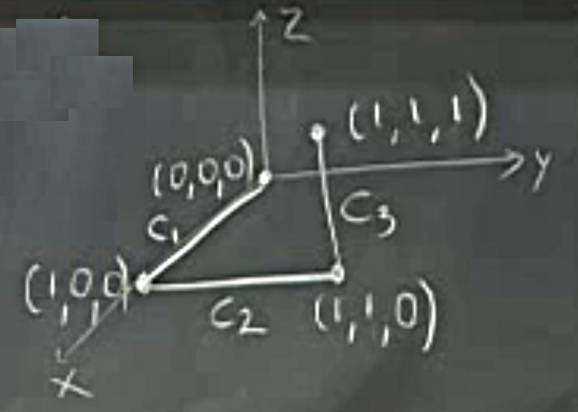
\includegraphics[width=15em]{calc_multi_30_01.jpg}

Nihai entegral üç parça halinde yapılmalı, $\int_C = \int_{C_1} + \int_{C_2} + \int_{C_3}$. 

$C_1,C_2$ icin $z=0$ v $\ud z = 0$ cunku bu egri $xy$ duzleminde, o zaman 

$$
\int yz \ud x + xz \ud y + xy \ud z = 0
$$

$C_3$ icin $x=1,y=1$ ve $\ud x = 0, \ud y = 0$. 

$$
\int_{C_3} \vec{F} \cdot \ud \vec{r} =
\int_{C_3} xy \ud z = \int_{0}^{1} \ud z = 1
$$

O zaman tüm entegral şöyle,

$$
\int_C = \int_{C_1} + \int_{C_2} + \int_{C_3} = 0 + 0 + 1 = 1
$$

Şimdi ilginç bir nokta, eğer aynı nihai noktaya farklı bir eğri üzerinden
erişsek o eğri üzerinden hesaplanan çizgi entegrali aynı sonucu verir. Bu durum
aslında $F$'nin bir gradyan alanı, yani muhafazar olması ile alakalı. Eğer bir
alan gradyan alanı ise, aynen basit türevlerde olduğu gibi, Calculus'un Temel
Teorisi geçerlidir, türevin yol üzerindeki entegrali tümlenen fonksiyonun
başlangıç ve bitiş arasındaki farkına eşittir,

$$
\int_C \nabla f \cdot \ud \vec{r} = f(P_1) - f(P_2)
$$

Peki $\vec{F} = < yz, xz, xy >$ alanının bir gradyan alanı olduğundan emin
miyiz? Evet çünkü bu alana gradyan alarak erişebileceğimizi biliyoruz, bir
tahmin yaparsak mesela $\vec{F} = \nabla (xyz)$ ile. O zaman örneğimize dönersek
çizgi entegralini sadece bitiş ve başlangıç noktalarını kullanarak
hesaplayabiliriz, $f(1,1,1) - f(0,0,0)$, $1 - 0 = 1$.











[devam edecek]

\end{document}



